\documentclass[tikz,border=4pt]{standalone}
\usetikzlibrary{positioning, arrows.meta}

\tikzset{
  fmap/.style       = {draw, thick, minimum width=5mm},
  encoder/.style    = {fmap, fill=blue!12},
  bottleneck/.style = {fmap, fill=orange!25},
  decoder/.style    = {fmap, fill=teal!15},
  channels/.style   = {font=\scriptsize},
  image/.style      = {draw, thick, fill=gray!12, minimum size=16mm, align=center},
  flow/.style       = {->, font=\scriptsize},
  skip/.style       = {->, dashed, draw=black!55},
  >={Stealth[length=2mm]},
}

\begin{document}
% A 2D encoder-decoder (U-Net-like). Each box is a feature map: its height shows
% the resolution, the number under it the channels. Skip connections run on top.
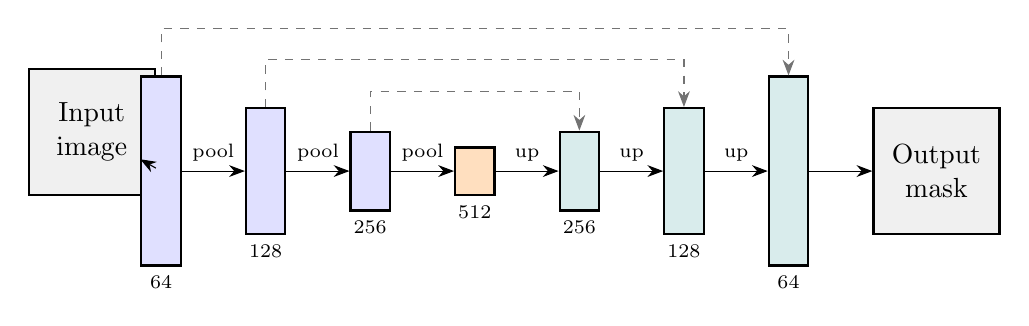
\begin{tikzpicture}[node distance=8mm]
  \node[image]                                                                    (in) at (1,0.5)  {Input\\ image};
  \node[encoder, minimum height=24mm, label={[channels]below:64}]     (e1) at (1.88,0)  {};
  \node[encoder, minimum height=16mm, label={[channels]below:128}, right=of e1]    (e2)  {};
  \node[encoder, minimum height=10mm, label={[channels]below:256}, right=of e2]    (e3)  {};
  \node[bottleneck, minimum height=6mm, label={[channels]below:512}, right=of e3]  (mid) {};
  \node[decoder, minimum height=10mm, label={[channels]below:256}, right=of mid]   (d3)  {};
  \node[decoder, minimum height=16mm, label={[channels]below:128}, right=of d3]    (d2)  {};
  \node[decoder, minimum height=24mm, label={[channels]below:64}, right=of d2]     (d1)  {};
  \node[image, right=of d1]                                                       (out) {Output\\ mask};

  \draw[flow] (in)  -- (e1);
  \draw[flow] (e1)  -- node[above] {pool} (e2);
  \draw[flow] (e2)  -- node[above] {pool} (e3);
  \draw[flow] (e3)  -- node[above] {pool} (mid);
  \draw[flow] (mid) -- node[above] {up} (d3);
  \draw[flow] (d3)  -- node[above] {up} (d2);
  \draw[flow] (d2)  -- node[above] {up} (d1);
  \draw[flow] (d1)  -- (out);

  % Skip connections: each encoder level to the decoder level of the same size.
  \draw[skip] (e3.north) -- ++(0,5mm) -| (d3.north);
  \draw[skip] (e2.north) -- ++(0,6mm) -| (d2.north);
  \draw[skip] (e1.north) -- ++(0,6mm) -| (d1.north);
\end{tikzpicture}
\end{document}
